% Results. Every number is a macro from generated/numbers.tex; every
% qualitative statement tagged "% claim: <name>" is checked against
% generated/claims.json by scripts/check_paper.py.

\begin{table*}[t]
\centering
\caption{Results at S3 (240 vehicles, 80\% penetration; IEEE 33-bus; \GEvalDays{} held-out days; learned methods averaged over \GTrainSeeds{} training seeds). Cost is the daily energy cost with its 95\% bootstrap confidence interval; Retail is the mean retail price paid (\euro/kWh); SQ is the delivered share of requested energy. ``+L3'' attaches the Level-3 layer to a baseline.}
\label{tab:main}
\footnotesize
\begin{tabular}{@{}lrrrrrrr@{}}
\toprule
Method & Cost (\euro) & Cost/kWh & Retail & SQ & Viol.\ (\%) & Mean $V^{\min}$ & Curt.\ (kWh) \\
\midrule
Uncoordinated & 931.4 {\scriptsize[833.8, 1060.7]} & 0.1146 & 0.200 & 1.000 & 3.99 & 0.9554 & 0.0 \\
Uncoordinated + L3 & 931.4 {\scriptsize[835.0, 1062.6]} & 0.1146 & 0.200 & 1.000 & 0.00 & 0.9615 & 5.0 \\
TOU timer & 697.7 {\scriptsize[639.6, 751.2]} & 0.0863 & 0.132 & 0.995 & 4.30 & 0.9372 & 0.0 \\
TOU timer + L3 & 697.1 {\scriptsize[641.0, 750.9]} & 0.0862 & 0.132 & 0.995 & 0.00 & 0.9515 & 23.7 \\
Price-aware heuristic & 619.8 {\scriptsize[561.8, 674.2]} & 0.0766 & 0.200 & 0.997 & 0.73 & 0.9598 & 0.0 \\
Price-aware heuristic + L3 & 619.8 {\scriptsize[564.4, 675.0]} & 0.0766 & 0.200 & 0.997 & 0.00 & 0.9623 & 1.7 \\
MPC LP-OPF (perfect foresight) & 612.0 {\scriptsize[555.7, 667.2]} & 0.0759 & 0.200 & 0.992 & 0.01 & 0.9634 & 0.0 \\
MPC LP-OPF (perfect foresight) + L3 & 612.0 {\scriptsize[555.3, 667.3]} & 0.0759 & 0.200 & 0.992 & 0.00 & 0.9635 & 0.0 \\
\midrule
Flat DDPG & 756.1 {\scriptsize[695.5, 828.3]} & 0.0934 & 0.203 & 0.996 & 0.45 & 0.9673 & 0.0 \\
Flat DDPG + L3 & 756.1 {\scriptsize[694.6, 827.0]} & 0.0934 & 0.203 & 0.996 & 0.00 & 0.9686 & 0.1 \\
PPO-Lagrangian & 790.2 {\scriptsize[725.8, 866.6]} & 0.0976 & 0.199 & 0.996 & 0.19 & 0.9758 & 0.0 \\
PPO-Lagrangian + L3 & 790.2 {\scriptsize[725.2, 865.0]} & 0.0976 & 0.199 & 0.996 & 0.00 & 0.9763 & 0.0 \\
CPO & 816.9 {\scriptsize[747.5, 900.1]} & 0.1006 & 0.200 & 0.999 & 0.35 & 0.9731 & 0.0 \\
CPO + L3 & 817.0 {\scriptsize[748.1, 903.3]} & 0.1006 & 0.200 & 0.999 & 0.00 & 0.9739 & 0.0 \\
Hierarchical RL & 741.3 {\scriptsize[685.3, 799.4]} & 0.0915 & 0.200 & 0.997 & 0.03 & 0.9741 & 0.0 \\
Hierarchical RL + L3 & 741.3 {\scriptsize[685.3, 800.0]} & 0.0915 & 0.200 & 0.997 & 0.00 & 0.9743 & 0.0 \\
\midrule
Nested (proposed) & 645.0 {\scriptsize[590.0, 700.0]} & 0.0797 & 0.201 & 0.997 & 0.00 & 0.9665 & 0.4 \\
\bottomrule
\end{tabular}

\end{table*}

\subsection{Main comparison}
\label{sec:res-main}
Table~\ref{tab:main} compares all methods at S3. Uncoordinated charging costs
\GUncoordinatedSThreeCost~\euro{} per day and violates the voltage floor in
\GUncoordinatedSThreeViol\% of the \SI{60}{s} steps.% claim: unc_violates_main
\ Attaching Level~3 removes every violation of the rule-based methods at
S1, S2, S3 and S5% claim: l3_zero_viol_rules_nominal
\ without changing their cost, because the correction uses reactive power and
curtails only when the headroom is exhausted. The perfect-foresight LP-OPF is
the cheapest method (\GLpOpfLThreeSThreeCost~\euro).% claim: lp_cheapest_S3
\ Among the methods that do not see the future, the price-aware heuristic is
cheapest (\GPriceAwareLThreeSThreeCost~\euro).% claim: pa_cheapest_nonoracle_S3
\ The nested controller costs \GNestedSThreeCost~\euro, which is
\GSavingNestedUncSThree\% less than uncoordinated charging and
\GGapNestedPaSThree\% more than the price-aware heuristic,% claim: pa_cheaper_than_nested_all_main
\ with no violations,% claim: nested_zero_viol_nominal
\ a service quality of \GNestedSThreeSq{} and a mean retail price of
\GNestedSThreeRetail~\euro/kWh. It is the cheapest learned controller,
\GSavingNestedBestLearnedSThree\% below the best learned baseline
(\GBestLearnedSThree).% claim: nested_cheapest_learned_main


\begin{table*}[t]
\centering
\caption{Daily energy cost (\euro) and violation rate (\%) across penetration levels S1--S5 (S4: S3 with \SI{15}{\percent} load-forecast error).}
\label{tab:scenarios}
\footnotesize
\begin{tabular}{@{}lrrrrrrrrrr@{}}
\toprule
Method & \multicolumn{2}{c}{S1 (40\%)} & \multicolumn{2}{c}{S2 (67\%)} & \multicolumn{2}{c}{S3 (80\%)} & \multicolumn{2}{c}{S4 (80\%)} & \multicolumn{2}{c}{S5 (100\%)} \\
 & Cost & Viol. & Cost & Viol. & Cost & Viol. & Cost & Viol. & Cost & Viol. \\
\midrule
Uncoordinated & 474 & 0.42 & 780 & 2.35 & 931 & 3.99 & 931 & 4.53 & 1161 & 6.82 \\
TOU timer & 358 & 0.06 & 587 & 2.39 & 698 & 4.30 & 695 & 4.31 & 858 & 7.55 \\
Uncoordinated + L3 & 474 & 0.00 & 780 & 0.00 & 931 & 0.00 & 931 & 0.02 & 1161 & 0.00 \\
TOU timer + L3 & 358 & 0.00 & 587 & 0.00 & 697 & 0.00 & 695 & 0.00 & 858 & 0.00 \\
Price-aware heuristic + L3 & 317 & 0.00 & 520 & 0.00 & 620 & 0.00 & 618 & 0.02 & 773 & 0.00 \\
MPC LP-OPF (perfect foresight) + L3 & 313 & 0.00 & 513 & 0.00 & 612 & 0.00 & 610 & 0.00 & 765 & 0.00 \\
Flat DDPG & 409 & 0.09 & 642 & 0.30 & 756 & 0.45 & 754 & 0.84 & 931 & 1.11 \\
PPO-Lagrangian & 403 & 0.01 & 662 & 0.16 & 790 & 0.19 & 788 & 0.62 & 984 & 0.51 \\
CPO & 420 & 0.03 & 684 & 0.27 & 817 & 0.35 & 814 & 0.93 & 1016 & 0.81 \\
Hierarchical RL & 380 & 0.00 & 622 & 0.04 & 741 & 0.03 & 739 & 0.38 & 922 & 0.19 \\
Nested (proposed) & 329 & 0.00 & 540 & 0.00 & 645 & 0.00 & 642 & 0.00 & 806 & 0.00 \\
\bottomrule
\end{tabular}

\end{table*}

\begin{figure*}[t]
\centering
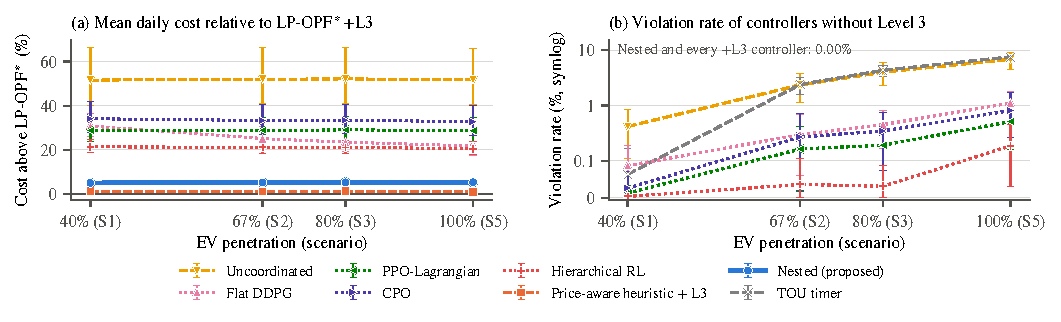
\includegraphics[width=\textwidth]{generated/fig_scenarios.pdf}
\caption{Cost per delivered kWh, service quality and violation rate across S1--S5 (means with 95\% bootstrap confidence intervals over days).}
\label{fig:scenarios}
\end{figure*}

\subsection{Penetration and forecast error}
\label{sec:res-scen}
Table~\ref{tab:scenarios} and Fig.~\ref{fig:scenarios} extend the comparison
to S1--S5. Without Level~3, violations of uncoordinated and TOU charging
grow with penetration, up to \GViolUncMax\% and \GViolTouMax\%.% claim: tou_violates_main
\ With accurate load forecasts (S1, S2, S3, S5) the nested controller and
every ``+L3'' method record no violations.% claim: nested_zero_viol_nominal
% claim: l3_zero_viol_rules_nominal
% claim: l3_zero_viol_learned_nominal
\ S4 is different: with a \SI{15}{\percent} base-load forecast error, the
household load alone breaks the floor on \GNoevViolDaysSFour{} of the
\GEvalDays{} days even when no vehicle charges. Level~3 removes most of these
violations with the reactive headroom of idle chargers ($\Qmax_i=S_i$ at
$P_i=0$); the remainder, at most \GViolNestedMaxSFour\% of the steps for the
nested controller, occurs only on those days.% claim: s4_l3_violations_only_base_load_days
\ The ordering of costs is the same at every penetration level: the nested
controller saves \GSavingNestedUncMin--\GSavingNestedUncMax\% relative to
uncoordinated charging, costs \GGapNestedPaMin--\GGapNestedPaMax\% more than the
price-aware heuristic, and stays below every learned baseline by at least
\GSavingNestedBestLearnedMin\%.% claim: nested_cheapest_learned_main


\begin{table}[t]
\centering
\caption{Paired comparison at S3: daily differences (nested minus method) with 95\% bootstrap intervals and Holm-corrected Wilcoxon signed-rank $p$-values.}
\label{tab:stats}
\footnotesize
\setlength{\tabcolsep}{3pt}
\begin{tabular}{@{}lrrrrr@{}}
\toprule
Nested vs. & $\Delta$Cost (\euro) & $p_{\mathrm{Holm}}$ & Days & $\Delta$SQ & $p_{\mathrm{Holm}}$ \\
\midrule
Uncoord. & -285.7 {\scriptsize[-376.8, -218.8]} & $<\!0.001$ & 50/50 & -0.0028 & $<\!0.001$ \\
Uncoord.+L3 & -285.7 {\scriptsize[-375.4, -219.4]} & $<\!0.001$ & 50/50 & -0.0028 & $<\!0.001$ \\
TOU & -52.0 {\scriptsize[-73.2, -32.7]} & $<\!0.001$ & 40/50 & +0.0014 & 0.070 \\
TOU+L3 & -51.3 {\scriptsize[-72.2, -32.4]} & $<\!0.001$ & 40/50 & +0.0016 & 0.019 \\
Price-aware & +25.9 {\scriptsize[+22.5, +29.8]} & $<\!0.001$ & 0/50 & +0.0001 & 1.000 \\
Price-aware+L3 & +25.9 {\scriptsize[+22.5, +29.8]} & $<\!0.001$ & 0/50 & +0.0001 & 1.000 \\
LP-OPF$^\ast$ & +33.7 {\scriptsize[+29.6, +38.5]} & $<\!0.001$ & 0/50 & +0.0046 & $<\!0.001$ \\
LP-OPF$^\ast$+L3 & +33.7 {\scriptsize[+29.6, +38.3]} & $<\!0.001$ & 0/50 & +0.0046 & $<\!0.001$ \\
Flat DDPG & -125.6 {\scriptsize[-157.5, -103.2]} & $<\!0.001$ & 50/50 & +0.0004 & 0.015 \\
Flat DDPG+L3 & -125.6 {\scriptsize[-157.4, -103.5]} & $<\!0.001$ & 50/50 & +0.0004 & 0.015 \\
PPO-Lag. & -151.4 {\scriptsize[-185.4, -124.8]} & $<\!0.001$ & 50/50 & +0.0009 & $<\!0.001$ \\
PPO-Lag.+L3 & -151.4 {\scriptsize[-185.8, -124.8]} & $<\!0.001$ & 50/50 & +0.0009 & $<\!0.001$ \\
CPO & -167.6 {\scriptsize[-212.3, -134.2]} & $<\!0.001$ & 50/50 & -0.0016 & $<\!0.001$ \\
CPO+L3 & -167.7 {\scriptsize[-211.2, -135.0]} & $<\!0.001$ & 50/50 & -0.0016 & $<\!0.001$ \\
HRL & -96.0 {\scriptsize[-106.7, -85.7]} & $<\!0.001$ & 50/50 & -0.0001 & 1.000 \\
HRL+L3 & -96.0 {\scriptsize[-106.9, -86.0]} & $<\!0.001$ & 50/50 & -0.0001 & 1.000 \\
\bottomrule
\end{tabular}

\end{table}

\subsection{Statistical comparison}
\label{sec:res-stats}
Table~\ref{tab:stats} tests the daily differences at S3. The cost differences
to uncoordinated charging and to every learned baseline are significant after
Holm correction,% claim: nested_sig_cheaper_all_learned_S3
\ and so is the cost premium relative to the price-aware heuristic% claim: nested_sig_costlier_than_price_aware_L3_S3
\ and the LP-OPF.% claim: nested_sig_costlier_than_lp_opf_L3_S3
\ The ``Days'' column counts the days on which the nested controller is the
cheaper of the pair.


\begin{table}[t]
\centering
\caption{Level-3 stress tests. S6 forbids charging from 19:00 to 20:00; S7 has 360 vehicles with inverters derated to 50\%. Violation rate (\%), minimum voltage (p.u.), curtailed and unmet energy (kWh per day) and service quality.}
\label{tab:stress}
\footnotesize
\setlength{\tabcolsep}{2pt}
\begin{tabular}{@{}lrrrrrr@{}}
\toprule
Method & \multicolumn{2}{c}{S6} & \multicolumn{4}{c}{S7} \\
\cmidrule(lr){2-3}\cmidrule(lr){4-7}
 & Viol. & $V_{\min}$ & Viol. & Curt. & Unmet & SQ \\
\midrule
Uncoord. & 3.80 & 0.951 & 9.00 & 0 & 6 & 1.000 \\
TOU & 4.32 & 0.937 & 10.62 & 0 & 402 & 0.968 \\
Uncoord.+L3 & 0.00 & 0.958 & 0.35 & 492 & 15 & 0.999 \\
TOU+L3 & 0.00 & 0.951 & 0.17 & 682 & 561 & 0.955 \\
Price-aware+L3 & 0.00 & 0.962 & 0.16 & 139 & 106 & 0.991 \\
LP-OPF$^\ast$+L3 & 0.00 & 0.963 & 0.00 & 0 & 98 & 0.992 \\
Nested & 0.00 & 0.966 & 0.01 & 46 & 38 & 0.997 \\
\bottomrule
\end{tabular}

\end{table}

\subsection{Level 3 under stress}
\label{sec:res-stress}
Table~\ref{tab:stress} probes Level~3 beyond nominal conditions. In S6 no
charging is allowed for an hour in the evening peak; because reactive headroom
is bounded by the inverter rating rather than by charging power, every
controller with Level~3 keeps the floor. S7 exceeds what halved inverters can
correct, and the methods separate. The nested controller curtails
\GReductionCurtNestedPaSSeven\% less energy than the price-aware heuristic,% claim: nested_less_curtailment_than_pa_S7
\ leaves \GReductionUnmetNestedPaSSeven\% less energy undelivered% claim: nested_less_unmet_than_pa_S7
\ and has \GReductionViolNestedPaSSeven\% fewer violations;% claim: nested_fewer_viol_than_pa_S7
\ its service quality is \GNestedSSevenSq{} against
\GPriceAwareLThreeSSevenSq.% claim: nested_higher_sq_than_pa_S7
\ The price of this robustness is energy cost: \GNestedSSevenCost~\euro{}
against \GPriceAwareLThreeSSevenCost~\euro{} per day.% claim: pa_cheaper_than_nested_S7


\begin{table}[t]
\centering
\caption{What the learned levels add (Level~3 active throughout). Plan: the Level-2 planning prior executed without learning; Prices only: learned corridor and execution prices with plan dispatch; Dispatch only: learned residual dispatch at the flat tariff. Daily cost (\euro), retail price (\euro/kWh), violations (\%), curtailed and unmet energy (kWh per day).}
\label{tab:decomp}
\footnotesize
\setlength{\tabcolsep}{2pt}
\begin{tabular}{@{}lrrrrrrr@{}}
\toprule
 & \multicolumn{3}{c}{S3} & \multicolumn{4}{c}{S7} \\
\cmidrule(lr){2-4}\cmidrule(lr){5-8}
Configuration & Cost & Retail & SQ & Cost & Viol. & Curt. & Unmet \\
\midrule
Price-aware+L3 & 619.8 & 0.200 & 0.997 & 940.4 & 0.16 & 139 & 106 \\
Plan+L3 & 627.9 & 0.200 & 0.997 & 956.7 & 0.02 & 114 & 37 \\
Prices only & 633.9 & 0.201 & 0.997 & 966.3 & 0.03 & 82 & 43 \\
Dispatch only & 645.3 & 0.200 & 0.998 & 981.4 & 0.03 & 71 & 30 \\
Nested & 645.0 & 0.201 & 0.997 & 982.9 & 0.01 & 46 & 38 \\
\bottomrule
\end{tabular}

\end{table}

\subsection{What the learned levels add}
\label{sec:res-decomp}
Table~\ref{tab:decomp} separates what each learned level contributes, with
Level~3 active throughout. Executed without learning, the plan costs
\GDecompCostVsPlanAbsPriceAwareLThreeSThree\% more at S3 than the per-vehicle
price-aware heuristic,% claim: decomp_price_aware_L3_cheaper_than_plan_S3
\ because the aggregate set point is filled least-laxity-first rather than by
each vehicle's own cheapest slots. Relative to the plan, learned prices alone
raise the S3 cost by \GDecompCostVsPlanAbsNestedPlanpriceSThree\%,% claim: decomp_nested_planprice_costlier_than_plan_S3
\ learned dispatch alone by \GDecompCostVsPlanAbsNestedFlatpriceSThree\%,% claim: decomp_nested_flatprice_costlier_than_plan_S3
\ and the full controller by \GDecompCostVsPlanAbsNestedSThree\%.% claim: decomp_nested_costlier_than_plan_S3
\ The learned dispatch spreads load away from the cheapest slots, which costs
energy at nominal load but pays off when the feeder is stressed: in S7 it
curtails \GDecompCurtVsPlanNestedFlatpriceSSeven\% less energy than the
plan% claim: decomp_nested_flatprice_less_curt_than_plan_S7
\ and leaves \GDecompUnmetVsPlanNestedFlatpriceSSeven\% less energy
undelivered.% claim: decomp_nested_flatprice_less_unmet_than_plan_S7

\begin{table}[t]
\centering
\caption{Ablations at S3 and S5 (daily cost in \euro, SQ, violation rate in \%).}
\label{tab:ablation}
\footnotesize
\setlength{\tabcolsep}{2.5pt}
\begin{tabular}{@{}lrrrrrr@{}}
\toprule
Configuration & \multicolumn{3}{c}{S3} & \multicolumn{3}{c}{S5} \\
 & Cost & SQ & Viol. & Cost & SQ & Viol. \\
\midrule
Complete framework & 645.7 & 0.997 & 0.00 & 806.6 & 0.997 & 0.00 \\
No planning prior & 696.5 & 0.996 & 0.00 & 865.5 & 0.996 & 0.00 \\
No Level 1 & 642.8 & 0.996 & 0.00 & 804.6 & 0.996 & 0.00 \\
Single timescale & 651.2 & 0.996 & 0.00 & 812.8 & 0.996 & 0.00 \\
No behavior model & 639.4 & 1.000 & 0.00 & 800.0 & 0.999 & 0.00 \\
No Level 3 (trained) & 648.5 & 0.996 & 0.23 & 810.5 & 0.995 & 0.71 \\
Level 3 removed at test & 645.7 & 0.997 & 0.33 & -- & -- & -- \\
No curriculum & 639.2 & 0.996 & 0.00 & 797.3 & 0.996 & 0.00 \\
No deadline guard & 651.2 & 0.996 & 0.00 & 814.6 & 0.996 & 0.00 \\
Proportional allocation & 660.8 & 0.995 & 0.00 & 828.5 & 0.995 & 0.00 \\
\bottomrule
\end{tabular}

\end{table}

\subsection{Ablations}
\label{sec:res-abl}

\begin{table}[t]
\centering
\caption{Generalization at 80\% penetration: second feeder, real ACN-Data sessions and the 2019 price regime (Unc.: uncoordinated; PA: price-aware; LP$^\ast$: perfect-foresight LP-OPF).}
\label{tab:general}
\footnotesize
\setlength{\tabcolsep}{2pt}
\begin{tabular}{@{}lrrrrrrr@{}}
\toprule
 & \multicolumn{4}{c}{Daily cost (\euro)} & \multicolumn{2}{c}{Viol.\ (\%)} & SQ \\
\cmidrule(lr){2-5}\cmidrule(lr){6-7}\cmidrule(lr){8-8}
Setting & Unc. & PA+L3 & LP$^\ast$+L3 & Nested & Unc. & Nested & Nested \\
\midrule
33-bus, residential & 931.4 & 619.8 & 612.0 & 645.0 & 3.99 & 0.00 & 0.997 \\
69-bus, residential & 931.4 & 619.8 & 611.7 & 648.0 & 0.21 & 0.00 & 0.997 \\
33-bus, ACN Caltech & 146.5 & 121.3 & 119.7 & 126.0 & 0.00 & 0.00 & 0.970 \\
33-bus, ACN JPL & 263.8 & 194.1 & 197.1 & 207.0 & 0.00 & 0.00 & 0.994 \\
33-bus, 2019 days & 371.1 & 282.3 & 280.2 & 289.9 & 4.72 & 0.00 & 0.997 \\
\bottomrule
\end{tabular}

\end{table}

\subsection{Generalization}
\label{sec:res-gen}

\begin{table}[t]
\centering
\caption{Sensitivity of Level 3 at S3 (nested controller): correction margin $\delta$ and inverter rating $S_i$ (default $\delta=0.001\pu$, $S_i=\SI{12}{kVA}$).}
\label{tab:sensitivity}
\footnotesize
\setlength{\tabcolsep}{3pt}
\begin{tabular}{@{}lrrrrr@{}}
\toprule
Setting & Cost (\euro) & SQ & Viol.\ (\%) & $Q$ act.\ (\%) & Curt.\ (kWh) \\
\midrule
$\delta = 0.0005$ & 645.7 & 0.997 & 0.000 & 0.36 & 0.5 \\
Default & 645.7 & 0.997 & 0.000 & 0.38 & 0.6 \\
$\delta = 0.002$ & 645.7 & 0.997 & 0.000 & 0.44 & 0.7 \\
$S_i = 10$ kVA & 645.8 & 0.997 & 0.000 & 0.38 & 4.7 \\
$S_i = 14$ kVA & 645.7 & 0.997 & 0.000 & 0.38 & 0.1 \\
\bottomrule
\end{tabular}

\end{table}

\subsection{Level-3 parameters}
\label{sec:res-sens}

\begin{figure*}[t]
\centering
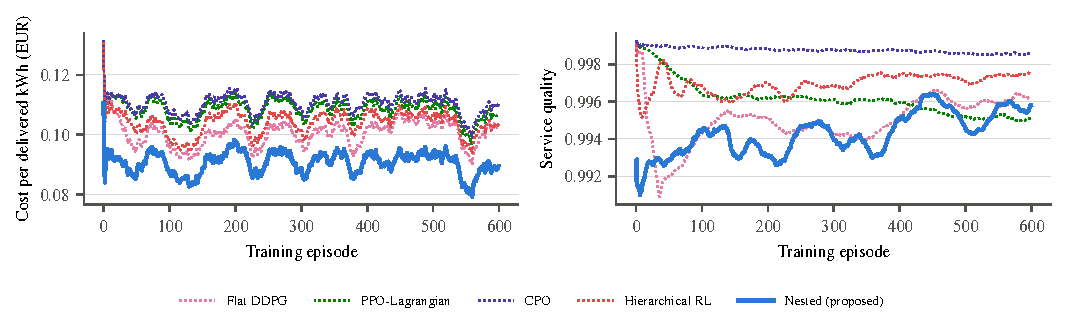
\includegraphics[width=\textwidth]{generated/fig_training.pdf}
\caption{Training curves (rolling mean over 25 episodes, averaged over seeds; exploration noise active).}
\label{fig:training}
\end{figure*}

\begin{table}[t]
\centering
\caption{Training cost on one CPU core per run.}
\label{tab:compute}
\footnotesize
\begin{tabular}{@{}lrrrr@{}}
\toprule
Method & Seeds & Episodes & s / episode & h / run \\
\midrule
CPO & 5 & 600 & 0.43 & 0.07 \\
Flat DDPG & 5 & 600 & 0.81 & 0.14 \\
Hierarchical RL & 5 & 600 & 2.69 & 0.45 \\
Nested (proposed) & 5 & 600 & 2.83 & 0.47 \\
PPO-Lagrangian & 5 & 600 & 0.35 & 0.06 \\
\bottomrule
\end{tabular}

\end{table}

\subsection{Training and computation}
\label{sec:res-comp}
